\section{Introduction}\label{sec:intro}
The choice of representation is a critical for learning a good generative model of 3D shapes. Voxel-based representations that discretize the geometric occupancy into a fixed resolution 3D grid offers compelling advantages since convolutional operations can be applied. 
However, they scale poorly with the resolution of the grid and are also wasteful since the geometry of most 3D shapes lies on their surfaces, resulting in a voxel grid that's mostly empty, especially at high resolutions. 
Surface-based representations such as triangle meshes and point clouds are more efficient for capturing surface geometry, but these representations are inherently unstructured -- because there is no natural ordering of the points, they are better expressed as an unordered \emph{set}. Consequently, unlike \emph{ordered} representations, they are cannot be easily generated using existing deep convolutional architectures. 
The exception is when the points are in perfect correspondence across shapes, in which case a linear shape basis can be effective (\eg, for faces or human bodies). However estimating accurate global correspondences is difficult and even poorly defined for categories such as chairs that have complex and varying geometry. Thus generating 3D shapes as point clouds remains a challenge.


We propose a new method for learning a generative model for 3D shapes represented as point clouds. Figure~\ref{fig:arch} illustrates our network architecture. 
The key idea is to use a space-partitioning data structure, such as a \emph{kd-tree}, to approximately order the points. 
Unlike a voxel-grid occupancy representation, the kd-tree representation scales linearly with the number of points on the surface and can adapt to the geometry of the model.
Moreover one can easily incorporate other point attributes such as surface normal, color, and texture coordinates into this representation, making it possible to generate new shapes that automatically include these information.
We learn a shape basis over the ordered point clouds using low-rank factorization of the shape coordinates. 
%The point cloud for each shape is optionally reordered such that the distance to the manifold spanned by the shape basis is minimized. 
%Subsequently a new shape basis can be learned on the reordered points and the process iterated till convergence.
If the alignments induced by the kd-tree sorting was perfect, the distribution of the coefficients would be simple.
Indeed this is the assumption behind generative models such as Probabilistic PCA~\cite{tipping1999probabilistic} that models the distributions of coefficients using independent Gaussians. 
However, imperfect alignment can lead to a multi-modal and heavy-tailed distribution over the coefficients.
To address this issue, we propose to leverage the expressive power of neural networks and employ a Generative Adversarial Network (GAN)~\cite{goodfellow2014generative} to learn the distribution over the shape coefficients.
Unlike other non-parametric distributions such as a mixture of Gaussians, the GAN linearizes the distribution of shapes and allows interpolation between them using arithmetic operations.
At the same time our method remains light-weight and scalable, since most shape categories can be well represented with a hundred basis coefficients.


\begin{figure}
\centering
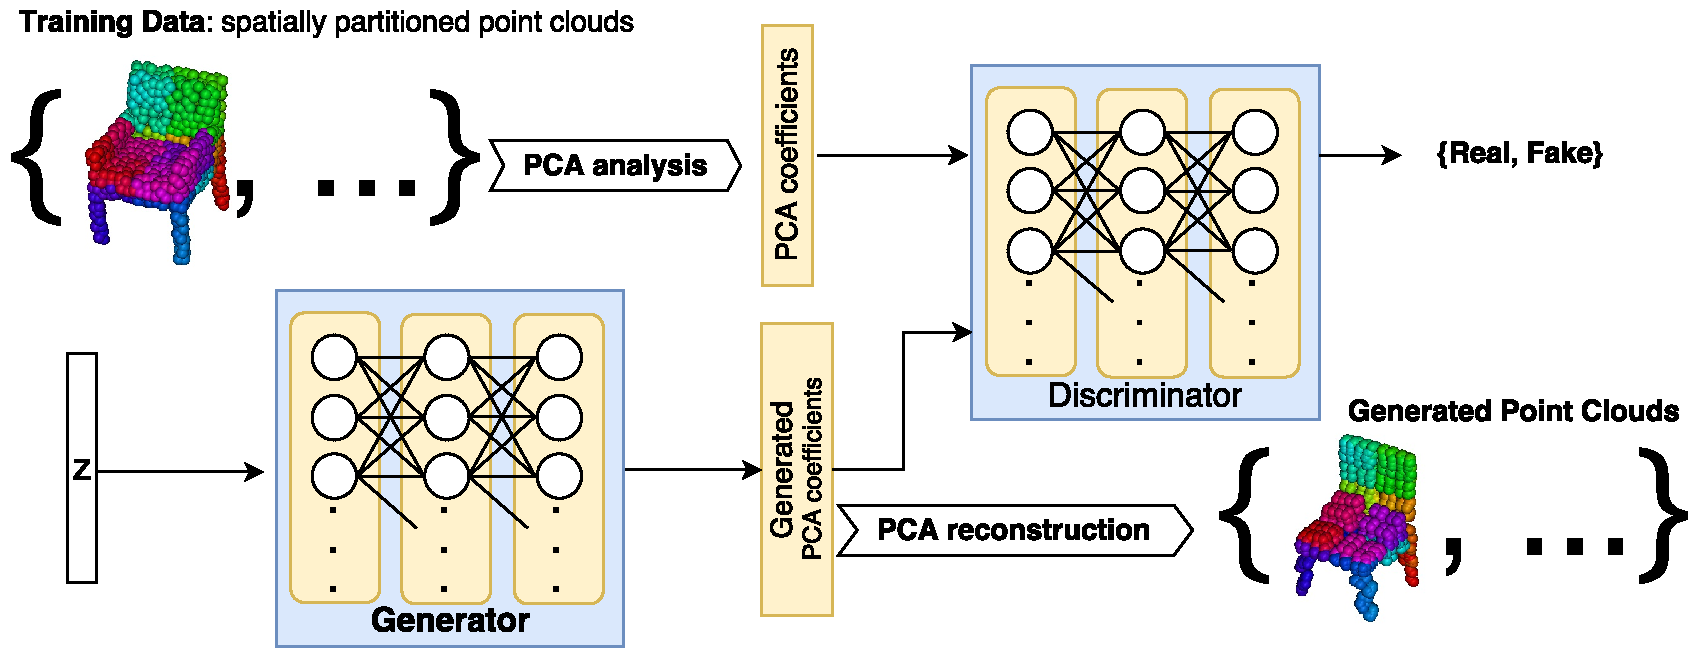
\includegraphics[width=0.8\linewidth]{PCAGAN/images/PCAGAN_architecture.pdf}
\caption{\small \label{fig:arch} Our network architecture for generating 3D shapes using spatially partitioned point clouds. We perform PCA analysis on the training data to drive a shape basis and associated shape coefficients. We then train a GAN to learn the multi-modal distribution over the coefficients. The generated coefficients are combined with the shape basis to produce the output point clouds.}
\vspace{-12pt}
\end{figure}

We compare the proposed generative model to a 3D-GAN approach of Wu~\etal~\cite{wu2016learning} that learns a convolutional architecture over a voxel-representation of 3D shapes. In addition we compare to a Probabilistic PCA (PPCA) baseline using the same point-cloud representation. Experiments on several categories in the ShapeNet dataset show that the proposed approach outperforms PPCA and 3D-GAN, quantitatively and qualitatively. Compared to the 3D-GANs our models are an order-of-magnitude faster and smaller. We then present several experiments evaluating the role of the kd-tree on the quality of the generated shapes. We also show that a 1D-convolutional GAN trained on the ordered list of point coordinates produces samples of reasonable quality, suggesting that the kd-tree ordering plays a key role.

